	\chapter{Kravspecifikation}
	
	\section{Aktør kontekst diagram}
		På Figur \ref{fig:AktorKontekst} ses aktør kontekst diagrammet for Rambøll Tilsyn. Diagrammet viser, hvilke aktører der interagerer med systemet.
	\begin{figure}[H]
		\centering
		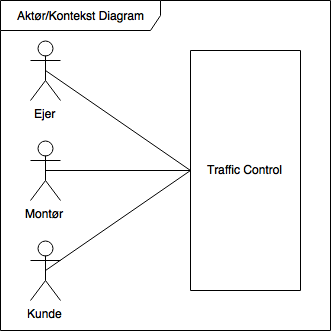
\includegraphics[width=0.6\linewidth]{Kravspecifikation/AktorDiagram}
		\caption{Aktør kontekst diagram for Rambøll Tilsyn.}
		\label{fig:AktorKontekst}
	\end{figure}

	På venstre side af Figur \ref{fig:AktorKontekst} ses brugeren, som er den primære bruger af systemet. Brugeren benytter systemet, som på diagrammet er symboliseret som en blackbox. På højre side, ses de sekundære aktører. Disse aktører er dem som systemet benytter sig af. Microsoft Office er en sekundær aktør, da systemet eksportere til Excel.
	
	\clearpage
	
\section{User stories diagram}
	Figur \ref{fig:Userstoriediagram} vises systemets User Stories diagram. Dette diagram viser den funktionalitet, som systemet indeholder beskrevet gennem en række User Stories, som beskrives i afsnit \ref{sec:UserS}.
	
	\begin{figure}[H]
		\centering
		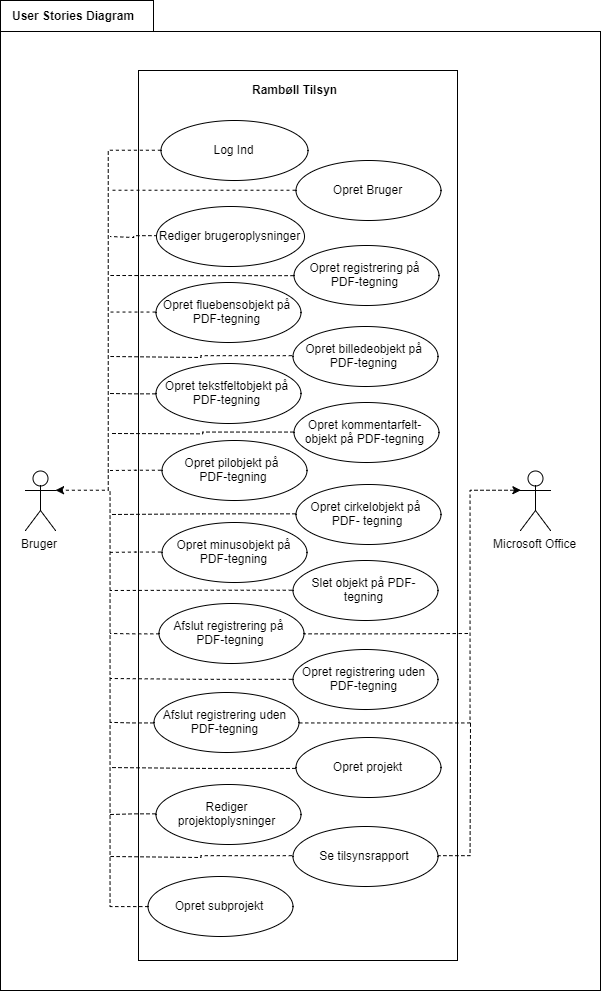
\includegraphics[width=0.6\linewidth]{Kravspecifikation/UserStorieDiagram}
		\caption{User Stories diagram for Rambøll Tilsyn.}
		\label{fig:Userstoriediagram}
	\end{figure}
	
	\clearpage
	
\section{Funktionelle krav} \label{sec:UserS}
	Følgende er en kort beskrivelse af udvalgte User Stories til Rambøll Tilsyn, som er fundet sammen med Rambøll ved hjælp af MoSCoW analyse \cite{MoSCoW}. For alle User Stories fuldt beskrevet med Gherkin, se Kravspecifikationens afsnit \ref{Krav-sec:UserStories} Funktionelle Krav.

	\subsection*{Log-in (CRS-1)}
	Denne User Story håndterer log-in på applikationen. Her skal brugeren indtaste korrekt brugernavn og kodeord, for at få adgang.
	
	\subsection*{Opret bruger (CRS-2)}
	Opret bruger User Storien giver en bruger mulighed for at oprette en ny bruger i systemet. Når brugeren er blevet oprettet, vil denne kunne logge ind på applikationen og benytte systemet.
	
	\subsection*{Opret en registrering på PDF-tegning (CRS-4)}
	Denne User Story håndterer det, at brugeren ønsker at oprette en registrering på PDF-tegning til et byggeprojekt.
	
	\subsection*{Opret fluebensobjekt på PDF-tegning (CRS-5)}
	I denne User Story får brugeren mulighed for, at sætte et flueben på PDF-tegningen i sin registrering. Fluebenet indikere at bruger har godkendt denne del af byggeriet.

	\subsection*{Opret billedeobjekt på PDF-tegning (CRS-6)}
	Denne User Story giver brugeren mulighed for, at tage et billede og placere på PDF tegningen. Når billedet er taget og placeret på PDF'en kan brugeren skrive en kort beskrivende tekst til billedet.
		
	\subsection*{Slet objekt på PDF-tegning (CRS-12)}
	I denne User Story får bruger mulighed for at slette et objekt. Hvis brugeren placerer et objekt forkert, eller kommer til at vælge det forkerte objekt, kan brugeren slette objektet. 

	\subsection*{Afslut registrering på PDF-tegning (CRS-13)}
	Denne User Story håndterer afslutningen af brugerens registrering. Når brugeren har oprettet alle objekter på PDF'en, kan der afsluts registrering ved tryk på 'Afslut' knappen og en excel-fil vil blive genereret med informationer om de forskellige objekter.
	
	\subsection*{Opret projekt (CRS-16)}
	Opret projekt User Storien giver brugeren mulighed for at oprette nye projekter i systemet. Når projektet er oprettet vil brugere kunne tilgå dette projekt og oprette registreringer. \\
	

\section{Ikke-funktionelle krav}
De ikke-funktionelle krav definerer de tekniske krav, som systemet skal indeholde. Disse krav beskriver egenskaber, som ikke har indvirkning på systemets funktionelle krav. Dette er eksempelvis antal brugere, der benytter systemet samtidig og hvordan brugerne skal have skrive og læse rettigheder. \\
Projektes ikke-funktionelle krav kan findes i afsnit \ref{Krav-sec:Ikkefunktionelle} i kravspecifikationen under bilag. \\

\section{Afgrænsning}
For at afgrænse projektet blev der holdt et møde med Rambøll, hvor de kunne komme med kommentar og ideer til systemet. \\
Der blev lavet en MoSCoW analyse til at prioritere funktionaliteten i systemet. Denne analyse form deler alt funktionaliteten op i fire kategorier \emph{must}, \emph{should}, \emph{could} og \emph{would}.
Det blev valgt at systemets \emph{must} User Stories definerer systemet og derved at disse funktionaliteter som er blevet implementeret i projektet, den detaljerede MoSCoW analyse kan findes i kravspecifikations Afsnit \ref{Krav-sec:MoSCoW} User stories, prioriteret efter MoSCoW. \\
Rambøll ønskede en applikation udviklet med fokus på iOS, da største delen af afdelingen har iPads tilknyttet. Der var dog en længere snak omkring dette, da også et par enkelte brugte Android. Derfor blev det aftalt, at der ville forsøges med at udvikle i cross-platform, som ville kunne fungere til både iOS og Android.
For den fulde afgrænsning samt MoSCoW analyse, henvises til Kravspecifikationens Afsnit \ref{Krav-sec:Afgraensning} Afgrænsning.
	